\subsubsection{Lifting decoder}\label{sec: lifting}
The Lifting decoder works as follows:
\begin{itemize}
    \item Create dual of Tanner graph
    \item Generate single-edge-colored subgraphs of the dual
    \item Decode subgraphs using MWPM/Union-Find
    \item Unify all edges from subgraph corrections
    \item Find all shortest-length loops on this union
    \item NOLIFTING CASE ????
    \item All nodes bounded by the faces that are elements of the shortest-length loop sets
    are error nodes. 
\end{itemize}
By sub-tiling
the graph into smaller subgraphs, we can reduce the problem of decoding
e.g. a honeycomb lattice toric color code to a set of
MWPM-decodable toric graphs that merely need to be "lifted" into a 
combination of subgraph decodings to decode the original color code
graph \cite{delfosse}. 
\begin{figure}[h!]
    \centering
    \subfigure[Original toric honeycomb lattice color code. Errors are marked yellow, \
    face colors are implied by opposing colors wrapping them.]{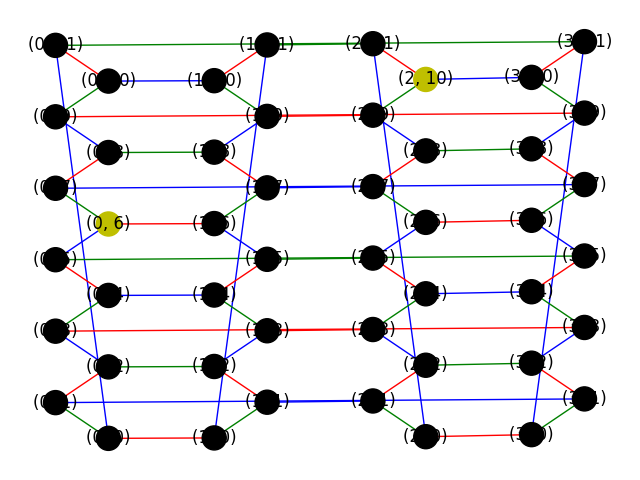
\includegraphics[width=0.4\textwidth]{img/figures/original.png}}\hfill
    \subfigure[Dual of color code lattice. Nodes are faces on the original lattice\
    yellow marked nodes represent syndromes.]{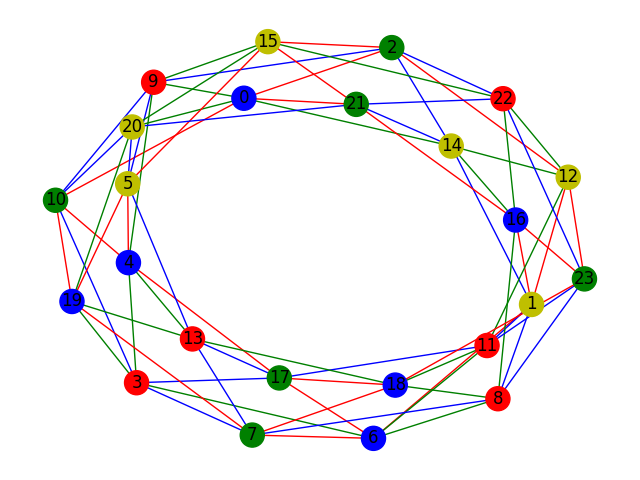
\includegraphics[width=0.4\textwidth]{img/figures/dual.png}}\hfill
    \subfigure[Red subgraph to be decoded via MWPM]{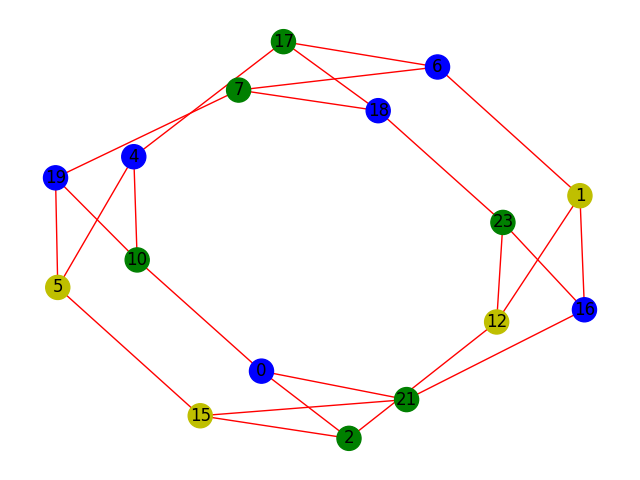
\includegraphics[width=0.4\textwidth]{img/figures/0.png}}\hfill
    \subfigure[Correct error prediction output for single distributed error nodes.]{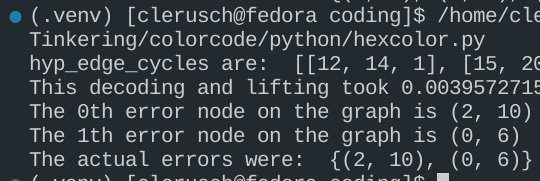
\includegraphics[width=0.4\textwidth]{img/figures/correctLiftingPred.png}}
    \caption{Steps in the lifting decoder. Generating code can be found in\ref{App: lifting}\
    and the entire git repository can be found in \cite{clemens}}
    \label{fig: lifting}
\end{figure}
This decoding is not optimal, as it does not take into account the other two colored
subgraphs when computing an MWPM edge prediction.
The polynomial time complexity of the lifting decoder does not
violate the NP-hardness of the 3-color matching problem, since the 
lifting procedure does not provide an optimal solution.
A graphical depiction of the steps of the lifting decoder is shown in
figure \ref{fig: lifting}.
\newpage